\chapter{Book I: the plates, and the lists that grew behind them}

\section{A Woolworth ledger}

The first of the three work books is the humblest object in the archive and the one that says most about how the record began. Its cover is a Woolworth \q{S. E. LEDGER}; its title page still carries the stationer's label, \q{HERALD SQUARE / Account Book / No. 2041 \ldots\ Made Expressly for F. W. Woolworth Co.}, and beneath the label, in her hand, the statement of method already quoted. The transcriber's note on that sheet is four words long and is the right response: \q{It says three books; six survive.} Inside the front cover a Berenice Abbott halftone portrait of the painter is hinged to the board; on the sheet after it, in drawn lettering the edition leaves unattributed, \q{Book I.}, and in her cursive, \q{From 1913} (\lfu{Book I}{title}{17616}; 16250).

The index on leaf 1 is the map of the volume and it is also the first evidence of a habit that runs through everything she wrote: the record is arranged, re-arranged and cross-referenced by its keeper, over decades, until the arrangement is itself a document. Etchings 2--47; Early Work, Paris Oils 50; Oils 52; Water colors by year 60--78; Notes 45--49; Etchings at Rehn 76; Current Exhibitions 84; Prizes 94--95; Reviews 98; Gifts 99; Reproductions 96--98; Photographs 92--93; and \q{Drawings} struck through with \q{+ Book IV for drawings} beside it, which is not the Book IV the Whitney numbered but the book of drawings the museum calls Book V (\lf{Book I}{1}{16800}). Beneath the page table is a two-column list of the etching plates with two prices against each, the second replacing the first; and in the margin, \q{More complete list for Carl \ill\ in \ill\ inside front cover - Feb. 14, 1961}, which is Carl Zigrosser of the Philadelphia Museum, a year before Philadelphia bought the whole output of the press.

On the same leaf stands the sentence the transcriber calls \q{the key to the whole of Book I}:

\begin{leafquote}
Notation in ink at right side of page is date when check received by E.H. from the Rehn Gallery. Pencil note means when picture sold to buyer.
\end{leafquote}

\noindent Ink is the cheque; pencil is the sale. It is a rule about media, and it means that the colour of the writing on these leaves carries information that a transcription in one typeface loses unless it says so. The edition says so, leaf by leaf, and this study depends on it.

\section{One plate to a leaf}

Leaves 2 to 44 hold the etchings, one plate to an odd leaf with the record continuing on the even leaf behind it. At the head of each is a halftone of the print, hinged; beside it the title and the plate size in Edward Hopper's drawn lettering, \q{the only words on this leaf in the other hand}, as the note on Evening Wind puts it (\lf{Book I}{2}{16853}). Then thirty or forty ruled lines in her hand, under headings that vary from leaf to leaf and are transcribed as they vary: Date, accepted / Refused, Exhibitions, Sold to and terms, Amount, when received; and below a red rule a second band for resales, \q{Date of sale / amt. rec'd / Sold by whom - to whom} (\lf{Book I}{18}{17168}).

What these leaves record, first of all, is a career of submission. The narrow column of \q{A} and \q{R} runs from a Los Angeles print jury in January 1921 through the Brooklyn Society of Etchers, the Chicago Society, the Print Club of Philadelphia, the National Academy of Design, and the refusals are entered as carefully as the acceptances. In the margin of the first plate leaf, in her hand, is the sentence that closes that career: \q{After 1926 nothing sent to juries} (\lf{Book I}{2}{16853}). Rehn had taken him on in the autumn of 1924; by 1926 the juries were no longer needed.

The prices tell the same story in figures, and they are worth setting out because they are the clearest series in the archive. In 1919 Les Poilus went to Carl Smalley for eight dollars (\lf{Book I}{41}{18062}). In 1921 the Monhegan Boat went to the State Library at Los Angeles for eighteen, of which \$16.20 arrived; the Bull Fight was \q{\$22 - 10\%} in May of that year; Les Deux Pigeons sold at Weyhe's book shop at \q{\$15 - 40\%}, nine dollars to the artist (\lf{Book I}{40}{17668}). In 1922 and 1923 the discounts are the story: Mrs. Sterner \q{30\% out of 18} = 12.60; Sidney Phillips \q{\$18 - 50\%} = 9; the Brooklyn Museum \q{\$22 - 15\%} = 18.70; House Tops at \q{\$15 - 33 1/3\%} = \$10 and, at the Whitney Studio Club, \q{No commission 15} (\lf{Book I}{32}{16428}). In 1924 the New Republic paid \q{Use of plate \$100} and \q{Royalties 150} for the portfolio (\lf{Book I}{6}{16548}). In May 1925 the Metropolitan bought fifteen etchings as a group through William Ivins at ten dollars a print, an accession the museum still lists as lot 25.31. From 1927 the terms settle at a third to the dealer on twenty-five dollars, \q{25 - 1/3} = 16 2/3, and in the autumn of 1929 at thirty, \q{30 - 1/3} = 20, which is what an impression of Evening Wind or Night Shadows cost for the next twenty years. In 1945, \q{Price raised to 50 - last few prints of Edition} (\lf{Book I}{3}{17443}). In June 1949 the Carnegie bought eleven prints for \$300, \q{average of 27.27 - 1/3 Rehn Gal. = \$18}; and on 2 February 1962 the Philadelphia Museum bought, as she wrote on leaf 44, the \q{large collection of etchings \& dry points in various states}, with seven preliminary drawings valued at five and six hundred dollars each, which the transcriber observes are \q{the only figures in Book I that are not sale prices, and they are forty times the prices on the leaves around them} (\lf{Book I}{44}{18288}).

Forty years, then, from eight dollars to thirty, and the plate itself, when a museum finally valued it, at six hundred. An etcher's economy is small and the book knows it. One leaf records a sale to the British Museum, in pencil, in a later hand: \q{Given to Fuller Brush man, friend of \unc{Rabbitfoot} - queer Dick - Sold Etching of E.H. - Night Shadows to British Mus. \ldots\ 1£ - then \$5 - so it could be listed as a sale. \ldots\ Curator there liked etching but no funds to buy} (\lf{Book I}{89}{18152}). A pound and then five dollars, so that it could be listed as a sale: the sentence is about the record as much as about the money, and it is one of many places where she is visibly keeping the book for the museum that would one day read it.

Her own queries about her own bookkeeping stand on the leaves. Beside a Weyhe row on leaf 7: \q{could this be a duplicate note?} (\lf{Book I}{7}{16439}). On the leaf of unlisted watercolours: \q{Could this be Shipyard, Rockland - schooner Butterfly? p. 64.} and, of Pretty Penny, \q{Owned by Jo Hopper?} (\lf{Book I}{72}{18117}). On the Rehn etchings leaf: \q{19 Etchings to Utica Art Soc. Rudolph Tandler - where are they now?} (\lf{Book I}{77}{18222}). These are not errors in the record; they are the record recording its own limits, and a reader who wants to know how reliable the ledgers are should begin with the fact that their keeper did not always know.

\begin{figure}[htbp]\centering
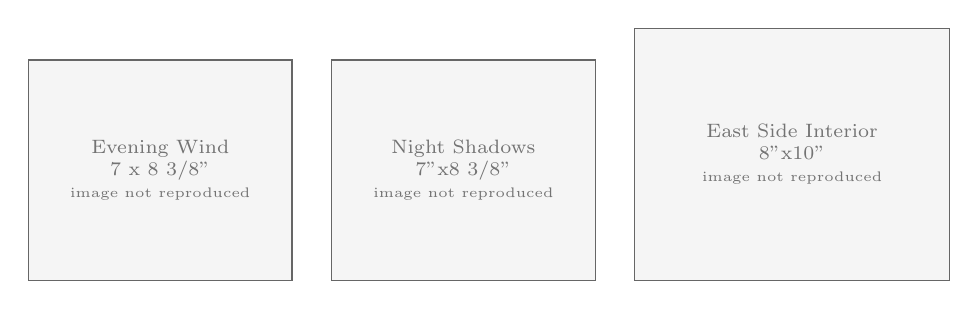
\begin{tikzpicture}
\draw[fill=black!4,draw=black!60,line width=0.5pt] (0,0) rectangle (3.35,2.8000000000000003);
\node[align=center,text=black!55,font=\scriptsize] at (1.675,1.4000000000000001) {Evening Wind\\7 x 8 3/8"\\\tiny image not reproduced};
\draw[fill=black!4,draw=black!60,line width=0.5pt] (3.85,0) rectangle (7.2,2.8000000000000003);
\node[align=center,text=black!55,font=\scriptsize] at (5.525,1.4000000000000001) {Night Shadows\\7"x8 3/8"\\\tiny image not reproduced};
\draw[fill=black!4,draw=black!60,line width=0.5pt] (7.7,0) rectangle (11.7,3.2);
\node[align=center,text=black!55,font=\scriptsize] at (9.7,1.6) {East Side Interior\\8"x10"\\\tiny image not reproduced};
\end{tikzpicture}
\caption{\textbf{Evening Wind}, etching, 1921, 7 x 8 3/8" as the leaf writes it (Book I, leaf 2, ref 16853). The Metropolitan Museum of Art, 25.31.7: \url{https://www.metmuseum.org/art/collection/search/366211}. \textbf{Night Shadows}, etching, 1921, 7"x8 3/8" as the leaf writes it (Book I, leaf 6, ref 16548). The Metropolitan Museum of Art, 25.31.2: \url{https://www.metmuseum.org/art/collection/search/366206}. \textbf{East Side Interior}, etching, 1922, 8"x10" as the leaf writes it (Book I, leaf 8, ref 17539). The Metropolitan Museum of Art, 25.31.1: \url{https://www.metmuseum.org/art/collection/search/366204}. Scale: ten inches to four centimetres, four times the scale of the canvases in the other figures. The frames are drawn to the proportions of the size in Edward Hopper's hand; the images are not reproduced here and can be seen at the museums' own pages. Drawn by Claude Fable~5.1, 13 September 2026, from the transcriptions and \texttt{works.json} (2026-09-13).}\label{fig:etchings}
\end{figure}


\section{The oils, written up afterwards}

From leaf 45 the volume changes character, and the change is instructive. She had a plate-by-plate book; she needed somewhere for everything else; and so the second half of Book I became, in no fixed order, a set of running lists: Notes and Explanations, Pre-Rehn Sales, Etching Collections, One Man Shows, Paris Paintings, Paris Watercolors, Oils 1913--1931 by year, Water Colors 1923--1931 by year, Etchings at the Rehn Gallery, Current Exhibitions 1923--1943, Reviews and Reproductions, Photographs, Prizes and Museum Purchases, Gifts, a page of accounts turned ninety degrees, and, on the back flyleaf, a chronology of the summers from 1923 to 1963. Several of these runs are bound back to front, because she filled a recto and then used the leaf before it for the overflow; the edition transcribes them in binding order and says so.

The oils leaves (52 to 59, 80 and 81) are where the early career is written up, and they are written up \emph{afterwards}: the watercolour leaves of 1924 to 1926 carry, in a later ink, the resales of June 1962, on rows first written forty years before. Here is the first canvas sold, twice over. On leaf 45: \q{Bought out of famous Armory Sale 1913 --- NewYork --- by --- Geo. Vietor. Sold by Arthur B. Davies.} and \q{This the first oil sold --- (turned up in fall of 1949 --- in different frame.)} On leaf 52, Sailing, \q{Sold at International Armory Show 1913 --- \$225} and then \q{Sold to Mr. Vietor, 25'' \& Mad. Ave. 250 - 10\%}, with \q{Sold by Arthur B. Davies} struck out (\lf{Book I}{52}{18056}). Book II gives \q{± \$250}, the dealers' book \$200, and the discrepancy is not a scandal: it is what a record made from memory looks like when it is made three times.

The oils prices climb where the etchings did not. Apartment Houses to the Pennsylvania Academy, \$340 net, 1925. House by a Railroad: \q{Price \$750, reduced to 600 - 1/3 Com. \$400} to Stephen Clark in March 1926, and on the line below, \q{Given to the Museum of Modern Art}, where it is accession 3.1930, credited \q{Given anonymously}. Sunday, \q{Bgt. by Duncan Phillips for \$600 !}, the exclamation hers. The Automat, 1200 less a third in 1927, 800 to the painter. Two on the Aisle, 1500 and 1000. Blackwell's Island, 2500 and 1666.67 in 1929. Tables for Ladies to the Metropolitan, \q{4500 - 1/3 3000 June 3, 1931}. Early Sunday Morning, then still \q{7th Ave. Shops} with \q{later named Early Sun. Morning} in her hand, 3000 less a third, 2000, to the Whitney on 5 May 1934. And in the 1950s the same leaves take the resales: Barber Shop to Roy Neuberger at \$4000 in 1954, Hotel Room to the Spingolds at 5500 in 1955.

On the Ex Lax leaf the descriptive habit becomes something else, an anecdote about a title:

\begin{leafquote}
It was suggested that E. Hopper change name to ES LAX. But the 2 X's in Ex Lax compose so much better, E. H. just made the change in water color. So soon after this, the canvas was bought by J. Spalding (Boston) who had no scruples about EX LAX, so water color S --- removed. But in meantime the picture had been photographed as Es Lax, \& reproduced somewhere, \& discovered by the Ex Lax people themselves, who wrote asking that the right name be used with their blessing. \hfill (\lf{Book I}{45}{16318})
\end{leafquote}

\noindent The two X's compose better: it is the painter's reason, reported by his wife, and it is the nearest thing in Book I to a statement of what he thought a picture was for.

Tables for Ladies gets the fullest description in the volume, and it shows the habit in its early, anecdotal form: \q{“Olga”, very blond, fine looking waitress all in white apron with bow in back. Cherry stained wood work + tiled floor. Cashier, Anna \unc{Popalgopalos} in black at desk, Max \unc{Scherer} + wife Sadie at table L. rear.} (\lf{Book I}{59}{16991}). The figures have names, and the names are hers; the transcriber marks two of them as doubtful readings, which is correct, but the doubt is about the letters and not about the fact that she named them. Capt. Ed Staples has a leaf of his own history: \q{“Honest Man in front of his Honest House” - Cleveland Plain Dealer - Summer 1929}, then \q{Burnt up in railroad accident on way back from Cleveland Museum - Summer 1929}, then \q{Insurance rec'd 2/3 assessed value 1000 Nov. 2 1929} (\lf{Book I}{55}{17525}). A watercolour that a buyer's wife would not have, Two Lights Village, is returned because \q{wife did'nt like out house} and exchanged for Civil War Camp Ground (\lf{Book I}{66}{16820}). Adam's House is \q{Presented to Frank + Peggy Rehn - Nov. 12, 1936. on the occasion of looking over the long list of sales made by them for E. H.} (\lf{Book I}{67}{17040}). Railroad Sunset: \q{A real beauty this one.} and \q{Given to Jo Hopper - along with Jo Painting - anniversary present 1955. Signed statement of this in bank box - J.H.} (\lf{Book I}{58}{18297}).

\begin{figure}[htbp]\centering
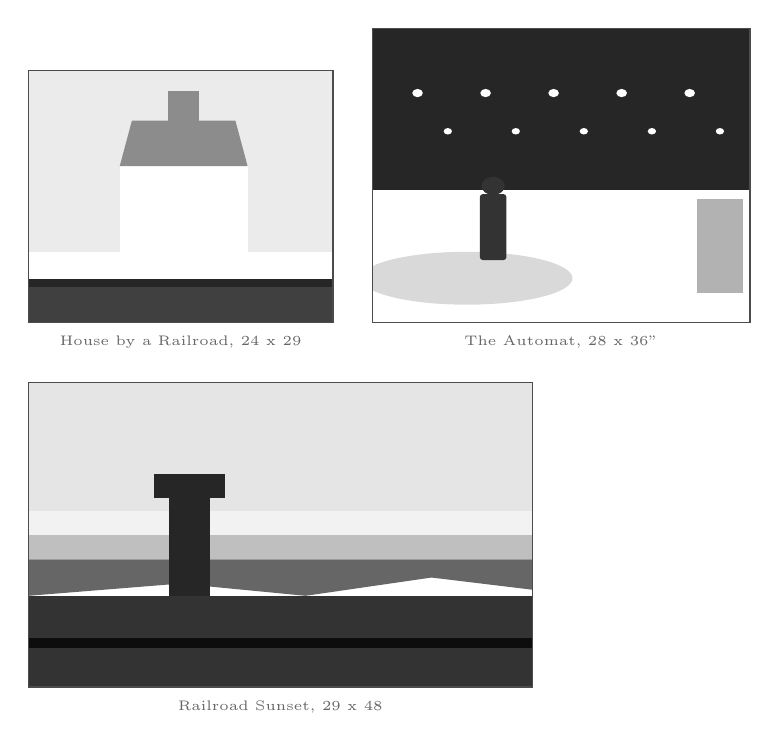
\begin{tikzpicture}
\begin{scope}[shift={(0,0)},x=3.867cm,y=3.200cm]\clip (0,0) rectangle (1,1);
\fill[black!8] (0,0.28) rectangle (1,1);            % sky
\fill[black!75] (0,0) rectangle (1,0.14);           % the embankment and rail
\fill[black!85] (0,0.14) rectangle (1,0.17);
\fill[white] (0.3,0.17) rectangle (0.72,0.62);      % the house
\fill[black!45] (0.3,0.62) -- (0.72,0.62) -- (0.68,0.8) -- (0.34,0.8) -- cycle; % mansard
\fill[black!45] (0.46,0.8) rectangle (0.56,0.92);   % the tower
\end{scope}
\draw[black!70,line width=0.5pt] (0,0) rectangle (3.8666666666666667,3.2);
\node[anchor=north,font=\tiny,text=black!60] at (1.9333333333333333,-0.05) {House by a Railroad, 24 x 29};
\begin{scope}[shift={(4.366666666666667,0)},x=4.800cm,y=3.733cm]\clip (0,0) rectangle (1,1);
\fill[black!85] (0,0.45) rectangle (1,1);            % the window, night
\foreach \x in {0.12,0.3,0.48,0.66,0.84} \fill[white] (\x,0.78) circle (0.014);
\foreach \x in {0.2,0.38,0.56,0.74,0.92} \fill[white] (\x,0.65) circle (0.011);
\fill[black!15] (0.25,0.15) ellipse (0.28 and 0.09); % table
\fill[black!80] (0.32,0.46399999999999997) circle (0.030799999999999998); \fill[black!80,rounded corners=1pt] (0.28500000000000003,0.21200000000000002) rectangle (0.355,0.436);
\fill[black!30] (0.86,0.1) rectangle (0.98,0.42);   % radiator
\end{scope}
\draw[black!70,line width=0.5pt] (4.366666666666667,0) rectangle (9.166666666666668,3.7333333333333334);
\node[anchor=north,font=\tiny,text=black!60] at (6.7666666666666675,-0.05) {The Automat, 28 x 36"};
\begin{scope}[shift={(0,-4.633333333333334)},x=6.400cm,y=3.867cm]\clip (0,0) rectangle (1,1);
\fill[black!10] (0,0.42) rectangle (1,1);          % sky, the sunset in bands
\fill[black!25] (0,0.42) rectangle (1,0.5);
\fill[black!5] (0,0.5) rectangle (1,0.58);
\fill[black!60] (0,0.3) -- (0.3,0.34) -- (0.55,0.3) -- (0.8,0.36) -- (1,0.32) -- (1,0.42) -- (0,0.42) -- cycle; % the dark hills
\fill[black!80] (0,0) rectangle (1,0.3);            % the embankment
\fill[black!95] (0,0.13) rectangle (1,0.16);        % the rails
\fill[black!85] (0.28,0.3) rectangle (0.36,0.62);   % the signal tower
\fill[black!85] (0.25,0.62) rectangle (0.39,0.7);
\end{scope}
\draw[black!70,line width=0.5pt] (0,-4.633333333333334) rectangle (6.4,-0.766666666666667);
\node[anchor=north,font=\tiny,text=black!60] at (3.2,-4.683333333333334) {Railroad Sunset, 29 x 48};
\end{tikzpicture}
\caption{\textbf{House by a Railroad}, oil, 1925; catalogued as House by the Railroad, 24 x 29 as the leaf writes it (Book I, leaf 52, ref 18056). The Museum of Modern Art, 3.1930: \url{https://www.moma.org/collection/works/78330}. \textbf{The Automat}, oil, 1927, 28 x 36" as the leaf writes it (Book I, leaf 54; Dealers, leaf 56). Des Moines Art Center, 1958.2: \url{https://desmoinesartcenter.org/wp-content/uploads/2022/04/cc-hopper.pdf}. \textbf{Railroad Sunset}, oil, 1929; « A real beauty this one. », 29 x 48 as the leaf writes it (Book I, leaf 58, ref 18297). Whitney Museum of American Art, work 5874: \url{https://whitney.org/collection/works/5874}. Scale: sixty inches to eight centimetres, the scale of every canvas frame in this note. The drawings are schemas of the composition in its main masses only, at the proportions of the size in Edward Hopper's hand, made from the leaf's description and from general knowledge of the picture; nothing is traced and no detail is drawn, and they are not reproductions. The pictures themselves are at the museums' own pages. Drawn by Claude Fable~5.1, 13 September 2026, from the transcriptions and \texttt{works.json} (2026-09-13).}\label{fig:bookioils}
\end{figure}


\begin{figure}[htbp]\centering
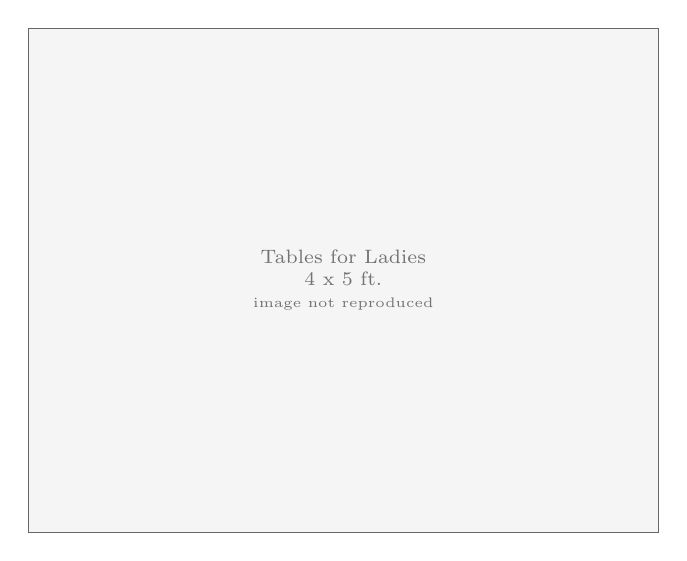
\begin{tikzpicture}
\draw[fill=black!4,draw=black!60,line width=0.5pt] (0,0) rectangle (8,6.4);
\node[align=center,text=black!55,font=\scriptsize] at (4,3.2) {Tables for Ladies\\4 x 5 ft.\\\tiny image not reproduced};
\end{tikzpicture}
\caption{\textbf{Tables for Ladies}, oil, 1930, 4 x 5 ft. as the leaf writes it (Book I, leaf 59, ref 16991). The Metropolitan Museum of Art, Hearn Fund, 1931: \url{https://www.metmuseum.org/art/collection/search/487695}. Scale: sixty inches to eight centimetres. The frames are drawn to the proportions of the size in Edward Hopper's hand; the images are not reproduced here and can be seen at the museums' own pages. Drawn by Claude Fable~5.1, 13 September 2026, from the transcriptions and \texttt{works.json} (2026-09-13).}\label{fig:tables}
\end{figure}


\section{Her own collection}

The signed statement in the bank box points to a thread that runs through all six books and is easy to miss: Josephine Hopper's own collection, and her anxiety that it should be recorded as hers. On leaf 47, under Etching Collections, she lists the impressions she owned: \q{these Etchings acquired as gifts for Xmas, birthday etc.}, dedicated \q{To my Wife or To Jo}, and \q{Left to show at Rehn Gallery after the Carnegie Inst. Show where they had been framed (\& mats trimming off !)}. On the Gifts leaf she returns to it: \q{They have been cut down (!) + framed by the Carnegie.} (\lf{Book I}{47}{18539}; \lf{Book I}{99}{17911}). Book V's loans page records one of her drawings \q{Owned by Jo N. Hopper for her collection}. In the dealers' book she writes of the same set: \q{All of this original group of 1933 Signed to my wife J.H.H. Should be full set, each given at some anniversary + set completed for Mod. Mus. show} (\lf{Dealers}{52}{17913}). These are the books of a woman who was also a painter, who knew what would happen to a collection nobody had documented, and who used her husband's ledgers to document hers.

The Gifts leaf has one more entry that belongs here because it points across the archive to the notebooks: \q{Night Shadows - Etching - May 1947 to Carl Hauptman - celebrating The Battle of Wash. Sq.}, and another impression to \q{Owen Grundy - of the Greenwich Villager who promoted the Battle of Wash. Sq.} (\lf{Book I}{99}{17911}). The fight with New York University over the house, which fills two of the four notebooks, was won, or was thought to have been won, in May 1947, and the ledger records the thank-you presents.

\section{Lists, and the money that vanishes}

The Current Exhibitions leaves (84 to 89) and the Reviews, Reproductions and Photographs leaves (90 to 93) hold ten leaves without a dollar sign, except the pound and the five dollars of the British Museum. The One Man Shows leaf gives the career in a column: 1919 Whitney Club; 1924 Rehn watercolours; 1926 St. Botolph's; 1927 and 1929 Rehn; 1932 Cleveland, guest of honour; 1933 Museum of Modern Art; 1934 the Arts Club of Chicago and the Fogg; 1937 Carnegie; 1941 Rehn, \q{Early Paintings 1907-1914}; 1948 Rehn; 1950 the Whitney retrospective, 13 February to 24 March, then Detroit; 1952 the Venice Biennale, \q{4 Americans \ldots\ E. Hopper, Stuart Davis, Kuniosti, Alex. Calder} (\lf{Book I}{49}{17717}). The Prizes leaves run from the Bryan and Logan prizes of \$25 each for East Side Interior in 1923 to the Corcoran's \q{1'' Prize of 2000 + Corcoran Gold Medal, Mar. 21'', 1937 - on Cape Cod Afternoon} and Chicago's \q{Ada S. Garrett prize \$750} for Night Hawks in 1942 (\lf{Book I}{94}{17837}; \lf{Book I}{95}{16884}).

The Reviews leaf has her reading the critics: \q{Reference to E.H. all the findings of the abstractionists there in E.H.}, of Edward Alden Jewell in the Times; \q{Forbes Watson speaks of E.H. as \unc{the} second best artist writer in America} (\lf{Book I}{96}{16426}). And it records the one fee he earned as a writer: \q{Review by E. Hopper --- for The Arts - Mar. 1926 (Rec'd check for \$13.30, Ap. 7, 26.} (\lf{Book I}{98}{18065}). The money returns on the last leaf, turned ninety degrees, in the accounts of the Rehn show of February 1927: advertising 161.50, window signs 3, photographs 44.80, frames for four oils 64, a frame for Two on the Aisle 20.74, ten watercolours 24.45, one etching 24, total 342.49; and against it the settlement of 4 November, \q{F. Rehn - 1452.68}: Two on the Aisle 1000, two watercolours 333.34, eight etchings 119.34 (\lf{Book I}{100}{17174}). The costs of the first one-man show at a commercial gallery were a quarter of what it brought in.

The back flyleaf is a chronology of summers, 1923 to 1963, and it is the skeleton of the life the notebooks flesh out: \q{1924 - near Bass Rocks '' married}; \q{1930 - Visit with Edward W. Root - Hamilton College, Clinton. No painting by E. H.}; \q{1934 - Built Studio house at S. Truro \ldots\ Not so much painting done - except watercolor of Jenness House}; 1941 the Pacific trip; 1943 and 1946 Mexico; 1948 \q{Rehn show, first hospital stay}; 1950 \q{diverticulosis}; \q{1962 - Truck burnt near Beach - Oct.}; 1963 the St. Botolph's award (\lfu{Book I}{flyleaf}{17234}). The years 1957 to 1959 are not written.

\section{What is lost, and what is doubtful}

A reader should know where Book I cannot be read. The hinged clippings are the chief loss: the Worcester halftone on leaf 2 hides every price from January 1921 to December 1922; leaf 56 is \q{the most nearly lost leaf}; the Camel's Hump halftone on leaf 81 is pasted flat with no second photograph. The Whitney's photographers turned some clippings back and photographed the leaf again, calling the second image a verso; the edition transcribes each table once, at the sheet where it can be read, and says which. The names that never settle are the buyers': Crowninshield is spelt three ways, Sheafer three, Spaulding two, Saltillo four. None is corrected, and the reason is the same as for the prices: a corrected name in a ledger is a claim about who bought a picture, and the leaf did not make it.

Only one reading in the entire volume is marked as checked by a person against the photograph: \q{Chicago}, first read \q{Shicago}, on leaf 8. That is the state of the edition, and this study inherits it.
